\hspace{-0.1in}
\tikzstyle{input_neuron}=[circle,draw=red!50,fill=red!10,thick,minimum size=5mm]
\tikzstyle{hidden_neuron}=[circle,draw=blue!50,fill=cyan!10,thick,minimum size=6mm]
\tikzstyle{output_neuron}=[circle,draw=green!50,fill=green!10,thick,minimum size=6mm]
\tikzstyle{bias_neuron}=[circle,draw=red!50,fill=red!10,thick,minimum size=2mm]
\tikzstyle{bias_hidden_neuron}=[circle,draw=blue!50,fill=cyan!10,thick,minimum size=2mm]

\tikzstyle{input}=[circle,draw=black!50,fill=black!20,thick,minimum size=6mm]

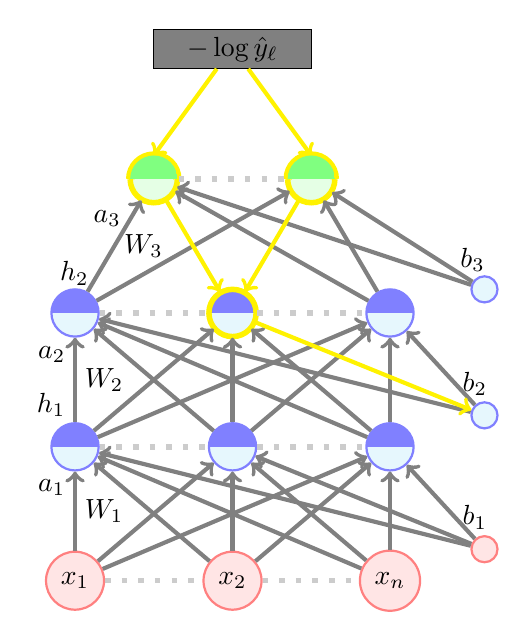
\begin{tikzpicture}
	\node [input_neuron] (neuron01) at (0,0) {$x_1$};
	\node [input_neuron] (neuron02) at (2,0){$x_2$};
	\node [input_neuron] (neuron03) at (4,0) {$x_n$};

	\node [bias_neuron] (neuron04) at (5.2,0.4) {};


	\node [hidden_neuron] (neuron11) at (0,1.7)  {};
	\node [hidden_neuron] (neuron12) at (2,1.7)  {};
	\node [hidden_neuron] (neuron13) at (4,1.7)  {};

	\node [bias_hidden_neuron] (neuron14) at (5.2,2.1) {};

	\begin{scope}
		\path[clip] (0,1.7) circle (3mm);
		\path[fill=blue!50] (-0.4,1.7) rectangle (0.3,2);
	\end{scope}
	\begin{scope}
		\path[clip] (2,1.7) circle (3mm);
		\path[fill=blue!50] (1.6,1.7) rectangle (2.3,2);
	\end{scope}
	\begin{scope}
		\path[clip] (4,1.7) circle (3mm);
		\path[fill=blue!50] (3.6,1.7) rectangle (4.3,2);
	\end{scope}


	\node [hidden_neuron] (neuron21) at (0,3.4)  {};
	\node [hidden_neuron] (neuron22) at (2,3.4)  {};
	\node [hidden_neuron] (neuron23) at (4,3.4)  {};

	\node [bias_hidden_neuron] (neuron24) at (5.2,3.7) {};


	\begin{scope}
		\path[clip] (0,3.4) circle (3mm);
		\path[fill=blue!50] (-0.4,3.4) rectangle (0.4,3.7);
	\end{scope}
	\begin{scope}
		\path[clip] (2,3.4) circle (3mm);
		\path[fill=blue!50] (1.6,3.4) rectangle (2.4,3.7);
	\end{scope}
	\begin{scope}
		\path[clip] (4,3.4) circle (3mm);
		\path[fill=blue!50] (3.6,3.4) rectangle (4.4,3.7);
	\end{scope}


	\node [output_neuron] (neuron31) at (1,5.1)  {};
	\node [output_neuron] (neuron32) at (3,5.1)  {};
	\draw [fill=gray] (1, 7) rectangle (3, 6.5) node[pos=0.5] {$-\log\hat{y}_\ell$};
	\draw [yellow,line width=1.5pt,  ->]   (1.8, 6.5) --(1,5.4);
	\draw [yellow, line width=1.5pt, ->]   (2.2, 6.5)-- (3,5.4);
	\draw[yellow, line width = 2] (1.7, 3.4) arc (180:360:3mm){};
	\draw [yellow, line width = 3] (1.3,5.1) arc (0:180:3mm) {};
	\draw [yellow, line width = 3] (3.3,5.1) arc (0:180:3mm) {};
	\draw[yellow, line width = 2] (0.7, 5.1) arc (180:360:3mm){};
	\draw[yellow, line width = 2] (2.7, 5.1) arc (180:360:3mm){};
	\draw[yellow, line width = 2] (2.3, 3.4) arc (0:180:3mm){};

	\begin{scope}
		\path[clip] (1,5.1) circle (3mm);
		\path[fill=green!50] (0.6,5.1) rectangle (1.3,5.4);
	\end{scope}
	\begin{scope}
		\path[clip] (3,5.1) circle (3mm);
		\path[fill=green!50] (2.6,5.1) rectangle (3.3,5.4);
	\end{scope}

	\draw[white,->] (neuron01) -- (neuron11) node[black,pos=.5,right]  {$W_{1}$} node[black,pos=0.8,left] {$a_{1}$};

	\draw[white,->] (neuron11) -- (neuron21) node[black,pos=.5,right] {$W_{2}$} node[black,pos=0.8,left] {$a_{2}$} node[black,pos=.2,left] {$h_{1}$};
	\draw[white,->] (neuron21) -- (neuron31) node[black,pos=.5,right] {$W_{3}$} node[black,pos=0.8,left] {$a_{3}$} node[black,pos=.2,left] {$h_{2}$};

	\draw[white,->] (neuron04) -- (neuron13) node[black,pos=0,right,above] {$b_1$};

	\draw[white,->] (neuron14) -- (neuron23) node[black,pos=0,right,above] {$b_2$};

	\draw[white,->] (neuron24) -- (neuron32) node[black,pos=0,right,above] {$b_3$};


	%\draw[white,->] (neuron31) -- (2.4.9) node[black,pos=1,above] {y };
	%\draw[white,->] (neuron31) -- (3,6.5) node[black,pos=1,above] {$f(x)$};
	%node[pos=1.3,above,right] {$\mathscr{L}(\theta)$};

	\draw[black!20,line width=2pt,loosely dotted] (neuron01) -- (neuron02);
	\draw[black!20,line width=2pt,loosely dotted] (neuron02) -- (neuron03);
	\draw[black!20,line width=2pt,loosely dotted] (neuron11) -- (neuron12);
	\draw[black!20,line width=2pt,loosely dotted] (neuron12) -- (neuron13);
	\draw[black!20,line width=2pt,loosely dotted] (neuron21) -- (neuron22);
	\draw[black!20,line width=2pt,loosely dotted] (neuron22) -- (neuron23);
	\draw[black!20,line width=2pt,loosely dotted] (neuron31) -- (neuron32);


	\foreach \from in {neuron01,neuron02,neuron03,neuron04}
	\foreach \to in {neuron11,neuron12,neuron13}
	\draw [black!50,line width=1.5pt,->] (\from) -- (\to);

	\foreach \from in {neuron11,neuron12,neuron13}
	\foreach \to in {neuron21,neuron23}
	\draw [black!50,line width=1.5pt,->] (\from) -- (\to);

	\foreach \from in {neuron21,neuron23, neuron24}
	\foreach \to in {neuron31,neuron32}
	\draw [black!50,line width=1.5pt,->] (\from) -- (\to);

	\draw [black!50, line width=1.5pt, ->] (neuron14)--(neuron21);
	\draw [black!50, line width=1.5pt, ->] (neuron14)--(neuron23);

	\draw [black!50, line width=1.5pt, ->] (neuron11)--(neuron22);
	\draw [black!50, line width=1.5pt, ->] (neuron12)--(neuron22);
	\draw [black!50, line width=1.5pt, ->] (neuron13)--(neuron22);

	\draw [yellow, line width=1.5pt, ->] (neuron22) -- (neuron14);
	\draw [yellow, line width=1.5pt, ->] (neuron31) -- (neuron22);
	\draw [yellow, line width=1.5pt, ->] (neuron32) -- (neuron22);

\end{tikzpicture}
